\chapter{Temperature and velocity distributions of a toy glacier and bedrock}

\modinfo{Directory}{ToyGlacierTemperatureAndFlow}
\modinfo{Solvers}{\Idx{HeatSolver},\Idx{FlowSolver}} 
\modinfo{Tools}{\Idx{ElmerGUI},\Idx{nglib}} 
\modinfo{Dimensions}{2D, Steady-state}
\modinfo{Author}{Thomas Zwinger, Peter R{\aa}back}


\subsection*{Introduction}

The purpose of this simple tutorial is to be an introduction into Elmer for people dealing with computational glaciology.
The tutorial is a continuation of the previous one with slightly more complex geometry. 
This tutorial shows how to apply two different solvers to two different bodies. 




\subsection*{Problem description}

Consider a 2D toy model of a glacier sitting an a piece of bedrock. 
With the bedrock present it is possible to study more accurately the temperature profiles. 

Now we solve for the temperature distribution $T$ for the combined system.
A heat flux of $q=0.02$~W/m$^2$ is applied at the bottom of the bedrock while the surface stays at a
fixed temperature of $T_0=-10$~C. For ice the properties from the database are assumed while for
the bedrock density is assumed to be 2500~kg/m$^3$ and heat conductivity 3~W/mK. 

We also solve for the velocity distribution $\vec{v}$ of the glacier. 
The velocity field is solved from the Stokes equation and is assumed to be affected only by the Gravity.
As boundary conditions we apply a no-slip condition at the ice-rock interface and symmetry condition at the right-hand-side of the glacier. 



\subsection*{Starting and meshing}

Start \texttt{ElmerGUI} from command line or by clicking the icon in your desktop (or in the /bin directory of you installation). 
Here we describe the essential steps in the ElmerGUI by writing out the clicking procedure. Tabulation generally means that the 
selections are done within the window chosen at the higher level. 

The mesh is given in ElmerGrid format in file \texttt{glacier\_on\_bedrock\_toy.in2d} in the samples directory of ElmerGUI, 
load this file.
\ttbegin
File 
  Open -> glacier\_on\_bedrock\_toy.in2d
\ttend
When netgen is ready with the meshing. You should obtain a mesh consisting of 4329 nodes and 8406
triangular elements. Now the mesh density was predefined in the \texttt{in2d} file and therefore no command-line
arguments are needed to refine the mesh. If you got more elements check the value of \texttt{Max H} in the netgen parameter window.

If the mesh was successfully imported your window should look something in figure~\ref{glacrock:mesh}.

\begin{figure}
\begin{center}
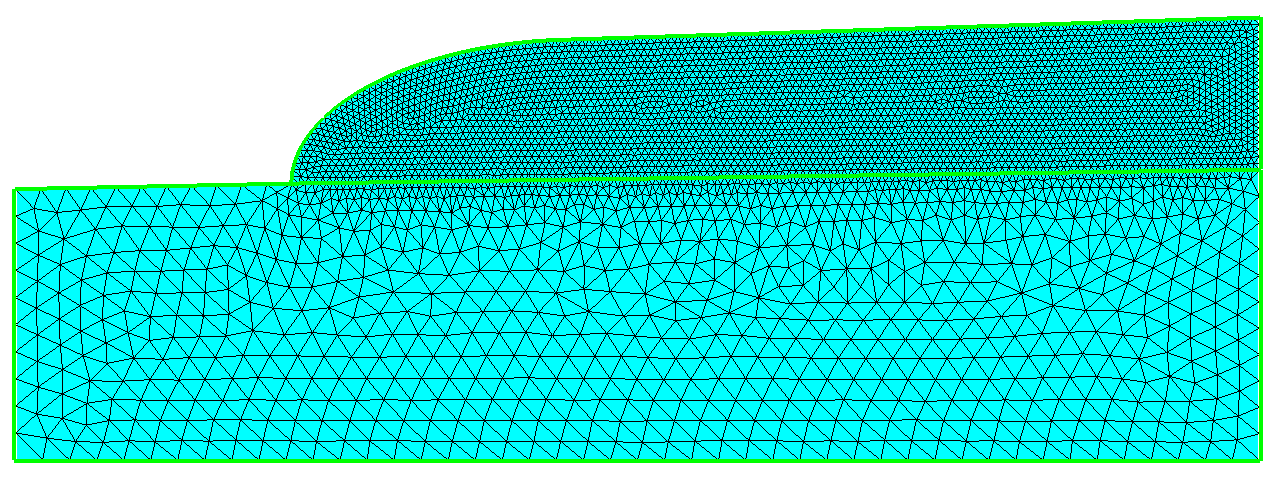
\includegraphics[width=120mm]{glacier_and_bedrock_toy_mesh}
\caption{The finite element mesh in ElmerGUI}\label{glacrock:mesh}
\end{center}
\end{figure}

\subsection*{Command file definition}

After we have the mesh we start to go through the Model menu from the top to bottom. 
Again we are happy with the definitions in the \texttt{Setup} window.

In the Equation section we choose the relevant equations and parameters related to their solution. 
In this case we'll have two different sets of solvers (called as Equation in Elmer slang). 
The first consists of heat and flow solvers, while the 
other includes just the heat solver. We'll name them appropriately. 

When defining Equations and Materials it is possible to assign to the bodies immediately, or to use mouse
selection to assign them later. In this case we know that the fluid body has the index 1 and the 
solid body has the index 2. Therefore it is easy to assign the Equation and Material to the bodies directly. 

Here we neglect the effect of convection to the temperature distribution. Therefore there is no coupling 
from velocity field to energy equation. However, the temperature is affecting the viscosity of ice and therefore
it needs to be solved first. This is ensured by giving higher priority to the heat solver
(default is zero). In order to obtain the Stokes equation convection of momentum is omitted 
from the Navier-Stokes equations.	

Here we are quite happy with the default solver settings of the individual equations of the linear systems.
However, the user may play around with different linear system settings to study their effect on 
convergence and computation time.
\\
The equation for the ice
\ttbegin
Model
  Equation
    Add
    Name = Heat and Flow
    Apply to Bodies = 1
    Heat Equation
      Active = on
      Priority = 1
      Convection = None
    Navier-Stokes 
      Active = on
      Convect = off
    OK
\ttend        
and then for the solid
\ttbegin
Model
  Equation
    Add
    Name = Just Heat
    Apply to Bodies = 2
    Heat Equation
      Active = on
      Convection = None
    OK
\ttend    

The Material section includes the material parameters.
We choose ice from the Material library which automatically sets for the needed material properties. 
For the bedrock we define the two parameters that are required. 
\ttbegin
Model
  Material
    Add 
      Material library
        Water (frozen)
      Apply to bodies = Body 1 
      Add 
      OK
    Add
      Name = Bedrock
      Apply to bodies = Body 2
      General    
        Density = 2500.0
      Heat Equation
        Heat Conductivity = 3.0
      Add
      OK
\ttend


A Body Force represents the right-hand-side of a equations. For the heat equation there are
no source terms. For the Stokes equation we apply gravity which
points to the negative $y$ direction.
\ttbegin
Model
  BodyForce
    Name = Gravity
    Navier-Stokes
      Force 2 = -9.81
    Apply to Bodies = Body 1 
    Add
    OK
\ttend

We do not need any Initial Condition since the zero temperature (in Celcius) is a good initial
guess for the heat equation. For the Stokes equation a better solution could be used since 
if convergence problems would arise since the non-Newtonian material laws do actually depend on the 
initial velocity.

We set four different kinds of boundary conditions. A fixed temperature, a fixed 
flux, no-slip condition and symmetry condition. As there are several boundaries
we first define the different boundary types, and thereafter assign them using the mouse.

\ttbegin
Model
  BoundaryCondition
    Add 
      Heat Equation
        Temperature = -10.0
      Name = Tsurface
      OK
    Add 
      Heat Equation
        Heat Flux = 0.02
      Name = Tflux
      OK
    Add 
      Navier-Stokes
        No-slip Wall BC = on
      Name = NoSlip
      OK
    Add 
      Navier-Stokes
        Velocity 1 = 0.0
      Name = Symmetry
      OK
\ttend   
Then we set the boundary properties 
\ttbegin
Model 
  Set boundary properties  
\ttend
Choose the correct boundary by clicking with the mouse
and apply the condition for this boundary.
\ttbegin
Boundary condition
  Click top boundary of ice -> choose Tsurface
  Click the bare part of bedrock -> choose Tsurface
  Click bottom boundary of bedrock -> choose Tflux
  Click bottom boundary of ice -> choose NoSlip
  Click r.h.s. boundary of ice -> choose Symmetry
\ttend

\subsection*{Saving and solution}

For the execution 
ElmerSolver needs the mesh files and the command file. We have now basically defined
all the information for ElmerGUI to write the command file. After writing it we may also visually 
inspect the command file.
\ttbegin
Sif 
  Generate
  Edit -> look how your command file came out  
\ttend

Before we can execute the solver we should save the files in a directory. In saving the project all the
necessary files for restarting the case will be saved to the 
destination directory.
\ttbegin
File 
  Save Project
\ttend

After we have successfully saved the files we may start the solver
\ttbegin
Run
  Start solver
\ttend
A convergence view automatically pops up showing relative changes of each iteration.
The heat conductivity of ice is set to be dependent on temperature and this results to a 
non-linear iteration.
The resulting output is shown in figure~\ref{glacrock:conv}.

\begin{figure}
\begin{center}
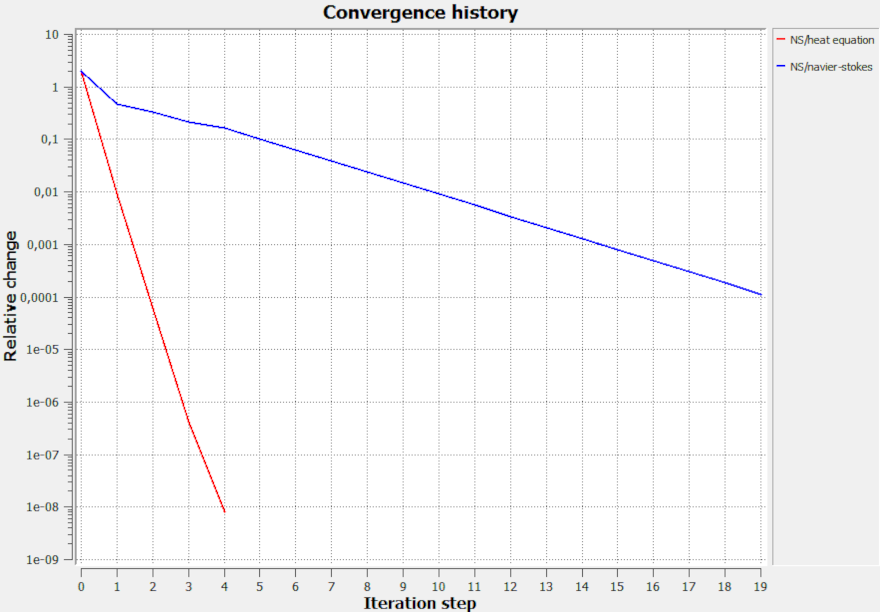
\includegraphics[width=100mm]{glacier_and_bedrock_toy_convergence}
\caption{The convergence  ElmerGUI}\label{glacrock:conv}
\end{center}
\end{figure}

Note: if you face problems in the solution phase and need to edit the setting, always remember to save
the project before execution.

\subsection*{Results}

To view the results we use Paraview,
\ttbegin
Run
  Start Paraview
\ttend
The resulting temperature and velocity distributions are shown in figure~\ref{glacrock:figtemp} (these are generated with the obsolete VTKPost tool within ElmerGUI).

\begin{figure}
\begin{center}
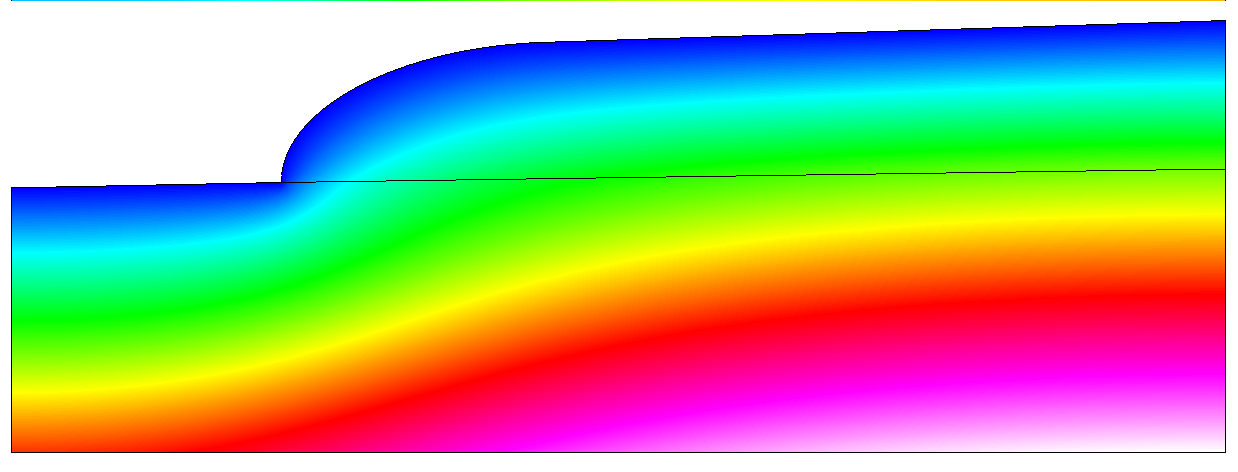
\includegraphics[width=120mm]{glacier_and_bedrock_toy_temp}
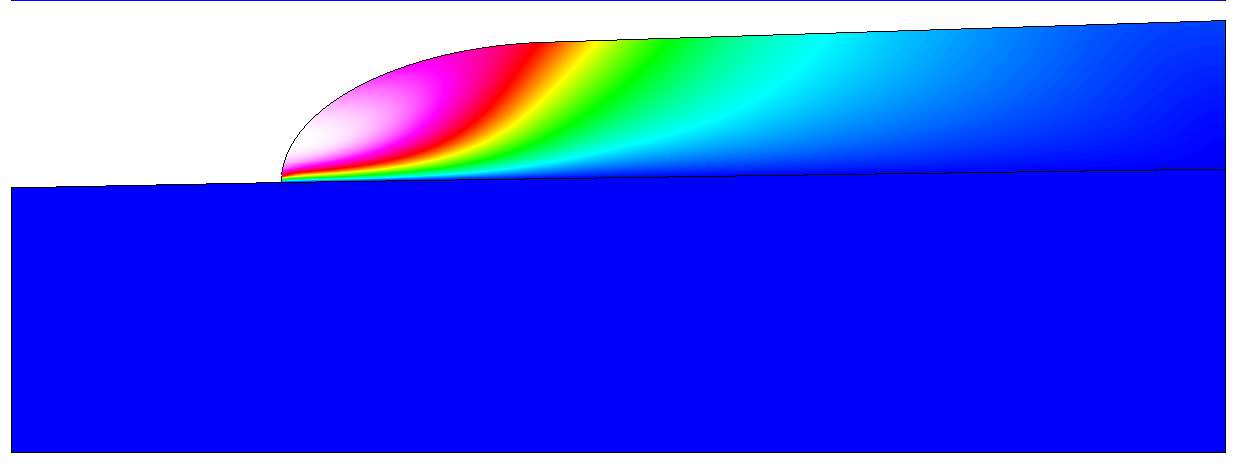
\includegraphics[width=120mm]{glacier_and_bedrock_toy_velo}
\caption{Temperature (upper figure) and velocity (lower figure) distributions 
of the toy glacier sitting on a bedrock.}\label{glacrock:figtemp}
\end{center}
\end{figure}


The maximum temperature obtained with the above choices is 12.955~C. 
For the velocity the maximum absolute value is 6.3337~mm/s which is actually unreasonably high since it 
corresponds to yearly movement of around 200~km. This just shows that the shape of the toy glacier 
under study is very unrealistic. 

\hfill
\mbox{}






